% Provenance (never printed): see sources/outline_sources.md (Year 1: elastic rebound and the
% seismic cycle; seismic moment and magnitudes; focal mechanisms; geodetic measurement of
% active deformation; the Gutenberg--Richter law). Exercise and problem values in the Book 3
% scratch calculator calc/ch18.py; figure data from figdata/bachelor-1/gutenberg_richter.py,
% beachballs.py and interseismic.py. Focus, epicentre, magnitude, intensity and seismometer
% are owned by Book 1 g7 (magnitude re-founded here as the moment magnitude); P and S waves by
% Book 2 g11; fault types and rake by ch. 17; stress, Coulomb and the seismogenic layer by
% ch. 16; the shear modulus by physics. Radar interferometry and the stereographic projection
% belong to later volumes (told, not defined).
\chapter{La source sismique}\label{ch:b1:earthquake-source}

% ledger: pp1515:1906, reid:1910
Le matin du 18 avril 1906, le sol au nord et au sud de San Francisco
s'est rompu le long d'une ligne de plus de quatre cents kilomètres. Routes, clôtures et
rangées d'arbres qui traversaient la ligne ont été coupées, et les deux moitiés de chacune ont été
trouvées à des mètres l'une de l'autre, la moitié ouest toujours déplacée vers le nord. Des arpenteurs
avaient mesuré les positions de repères dans la région durant le demi-siècle précédent, et quand les repères furent mesurés de nouveau la
comparaison montra quelque chose de plus étrange que la rupture elle-même~: le sol
s'était courbé, lentement et en douceur, pendant des décennies avant le séisme, et le
séisme l'avait laissé reprendre sa forme. Ce chapitre suit un séisme depuis
le lent chargement d'une faille jusqu'aux quelques minutes où elle glisse, et relit
le glissement dans les ondes et dans le sol~: quelle fut son ampleur, dans quelle
direction elle s'est déplacée, à quelle vitesse se prépare le suivant, et à quelle fréquence
viennent les séismes de chaque taille.

\begin{recall}
Le foyer d'un séisme est le point où la rupture commence, son
épicentre le point de la surface au-dessus de lui~; la magnitude mesure la taille
d'un séisme, l'intensité les secousses en un lieu~; un sismomètre enregistre
le mouvement du sol sous forme de sismogramme (livre~1, année~7). L'onde P, une
onde de compression, arrive la première et l'onde S, une onde de cisaillement, après elle
(livre~2, année~11). Une faille a un \omterm{def:b1:faults-folds-fabrics:fault-elements}{compartiment supérieur} et un \omterm{def:b1:faults-folds-fabrics:fault-elements}{compartiment inférieur}~; le \omterm{def:b1:faults-folds-fabrics:fault-elements}{vecteur glissement}
est le déplacement du \omterm{def:b1:faults-folds-fabrics:fault-elements}{compartiment supérieur} par rapport au \omterm{def:b1:faults-folds-fabrics:fault-elements}{compartiment inférieur}, son \omterm{def:b1:faults-folds-fabrics:fault-elements}{pitch}
$r$ est mesuré sur le plan de faille à partir de la direction, et le \omterm{def:b1:faults-folds-fabrics:fault-elements}{pitch} nomme la
faille~: environ \ang{90} inverse, environ \ang{-90} normale, environ 0 \omterm{def:b1:faults-folds-fabrics:fault-types}{senestre}, environ
\ang{180} \omterm{def:b1:faults-folds-fabrics:fault-types}{dextre} (\cref{ch:b1:faults-folds-fabrics}). Un solide élastique
retrouve sa forme quand la contrainte est retirée~; le module de cisaillement $\mu$
relie une contrainte de cisaillement à la \omterm{def:b1:stress-strain-rheology:strain}{déformation de cisaillement} qu'elle produit (physique)~; les failles glissent
quand la contrainte de cisaillement atteint leur résistance au frottement, et les séismes
commencent dans la partie cassante supérieure de la \omterm{def:b1:layered-earth:layers}{croûte}, la \omterm{def:b1:stress-strain-rheology:strength-envelope}{couche sismogène}
(\cref{ch:b1:stress-strain-rheology}). Des stations permanentes de positionnement par satellite,
dont les positions quotidiennes sur des années donnent la vitesse du sol là où elles
se trouvent, mesurent les mouvements des plaques (\cref{ch:b1:plate-kinematics}).
\end{recall}

\section{Rebond élastique et cycle sismique}\label{sec:b1:earthquake-source:cycle}

Deux plaques qui glissent l'une contre l'autre à vitesse constante ne glissent pas, en général,
régulièrement le long de la faille qui les sépare. Le frottement garde la faille bloquée
tandis que les plaques continuent de se déplacer loin d'elle, de sorte que les roches de part et d'autre sont
courbées comme un ressort. Quand la contrainte de cisaillement sur la faille atteint sa résistance,
la faille glisse en quelques secondes ou minutes, et les roches courbées reviennent brusquement.

\begin{definition}[Rebond élastique, cycle sismique, intervalle de récurrence]\label{def:b1:earthquake-source:seismic-cycle}
Le \emph{rebond élastique}\index{rebond elastique@rebond élastique} est le retour soudain vers
leur forme non déformée des roches de part et d'autre d'une faille, quand la faille,
bloquée tandis qu'elles étaient déformées, glisse lors d'un séisme~; l'énergie élastique
qu'elles avaient stockée est libérée, en partie sous forme d'ondes sismiques. Le \emph{cycle
sismique}\index{cycle sismique} d'un segment de faille est la séquence répétée d'un
long stade intersismique, pendant lequel le segment est bloqué et la déformation
s'accumule autour de lui, d'un stade cosismique, le séisme, pendant lequel il
glisse, et d'un stade postsismique, de mois à décennies, pendant lequel les
environs s'ajustent au nouvel état. L'\emph{intervalle de
récurrence}\index{intervalle de recurrence@intervalle de récurrence} d'un segment est le temps entre deux
grands séismes successifs sur lui.
\end{definition}
% ledger: usgs:gloss-rebound, reid:1910, usgs:pp1515-thatcher

\begin{omfigure}
\begin{tikzpicture}[>={Stealth[length=5pt]}, font=\small]
% map view of a fence across a locked dextral strike-slip fault (north up): (a) built straight;
% (b) after decades of loading, bent with the interseismic profile v(x) = -(s/pi) arctan(x/D)
% (dextral: the east side moves south); (c) after the earthquake, straight again on each side and
% offset by s at the fault. Panel 3.4 cm wide (x from -1.7 to 1.7 cm), D = 0.35 cm, s = 0.9 cm.
\def\s{0.9}\def\Dl{0.35}
\foreach \k/\t in {0/{(a) la clôture est construite}, 1/{(b) des décennies de chargement}, 2/{(c) après le séisme}} {
  \begin{scope}[xshift=\k*4.6cm]
    \fill[omLithSand!25] (-1.7,-1.6) rectangle (1.7,1.6);
    \draw[black!50, line width=0.4pt] (-1.7,-1.6) rectangle (1.7,1.6);
    \draw[fault, line width=1.1pt] (0,-1.6) -- (0,1.6);
    \node[anchor=north, align=center, font=\scriptsize] at (0,-1.7) {\t};
    % far-field motion of the two blocks, relative to the fault
    \draw[->, omThm, line width=0.8pt] (-1.35,-1.25) -- (-1.35,-0.45);
    \draw[->, omThm, line width=0.8pt] (1.35,1.25) -- (1.35,0.45);
    \ifnum\k=0
      \draw[line width=1.2pt, omDef] (-1.7,0) -- (1.7,0);
    \fi
    \ifnum\k=1
      \draw[line width=1.2pt, omDef] plot[domain=-1.7:1.7, samples=81, variable=\x] (\x, {-\s/pi*atan(\x/\Dl)*pi/180});
      \draw[black!45, dashed, line width=0.4pt] (-1.7,0) -- (1.7,0);
    \fi
    \ifnum\k=2
      \draw[line width=1.2pt, omDef] (-1.7,{\s/2}) -- (0,{\s/2});
      \draw[line width=1.2pt, omDef] (0,{-\s/2}) -- (1.7,{-\s/2});
      \draw[black!45, dashed, line width=0.4pt] (-1.7,0) -- (1.7,0);
      \draw[<->, line width=0.5pt] (0.18,{\s/2}) -- (0.18,{-\s/2});
      \node[anchor=west, font=\scriptsize] at (0.2,0.12) {glissement};
    \fi
  \end{scope}
}
\node[anchor=south, font=\scriptsize] at (0,1.62) {faille};
\draw[->, line width=0.5pt] (-1.5,0.75) -- (-1.5,1.15) node[above, font=\scriptsize, inner sep=1pt] {N};
\end{tikzpicture}
\par\smallskip{\small \omterm{def:b1:earthquake-source:seismic-cycle}{Rebond élastique} vu de dessus, sur une clôture (en bleu)
construite droite en travers d'une faille \omterm{def:b1:faults-folds-fabrics:fault-types}{dextre} bloquée. Flèches rouges~: le mouvement des
deux blocs loin de la faille, par rapport à elle. (b) Tant que la faille est bloquée,
le sol lointain bouge et la clôture se courbe, le long de la courbe du
profil intersismique de la \cref{sec:b1:earthquake-source:geodesy}. (c) Le
séisme libère la courbure~: chaque moitié de la clôture est de nouveau droite, et
les deux moitiés sont décalées à la faille du glissement. La courbure est
exagérée~: une vraie clôture se courbe de quelques mètres sur des dizaines de kilomètres.}
\label{fig:b1:earthquake-source:rebound}
\end{omfigure}

Si la faille est bloquée entre les séismes et que chaque séisme défait le
glissement accumulé par les plaques depuis le précédent, le mouvement des plaques fixe le
rythme du cycle.

\begin{proposition}[La récurrence à partir de la vitesse de glissement]\label{prop:b1:earthquake-source:recurrence}
Soit un segment de faille chargé à la vitesse de glissement à long terme $\dot s$, bloqué
entre les séismes, et glissant de la même quantité $D$ à chaque séisme. Alors
l'\omterm{def:b1:earthquake-source:seismic-cycle}{intervalle de récurrence} de ses séismes est
\[
  T = \frac{D}{\dot s} .
\]
Si seule la fraction $c$ de la vitesse de glissement est bloquée, le reste glissant
régulièrement sans séismes, $T = D/(c\,\dot s)$.
\end{proposition}

\begin{proof}
Sur un long temps $t$, les deux côtés de la faille se déplacent de $\dot s\,t$ l'un par rapport
à l'autre. Loin de la faille le sol bouge régulièrement, donc sur la faille
elle-même le même déplacement doit être rattrapé, ici par les seuls séismes~: si
$N$ séismes se produisaient dans le temps $t$, alors $N D = \dot s\,t$ au
glissement d'un séisme près, et $t/N \to D/\dot s$. Avec la fraction $1-c$ du
glissement faite par glissement régulier, les séismes rattrapent $c\,\dot s\,t$ et
$t/N \to D/(c\,\dot s)$.
\end{proof}

Avec des valeurs typiques de la faille de San Andreas, un glissement de \qty{4}{m} à chaque grand
séisme et une vitesse de glissement de \qty{20}{mm.an^{-1}}, l'\omterm{def:b1:earthquake-source:seismic-cycle}{intervalle de récurrence} est
de \qty{200}{ans}. À Wallace Creek, dans le centre de la Californie, un chenal de cours d'eau coupé
à travers la faille a été décalé de \qty{128}{m} en \num{3587} ans depuis
son incision, soit en moyenne \qty{36}{mm.an^{-1}}, proche de la vitesse d'environ
\qty{34}{mm.an^{-1}} mesurée sur d'autres décalages de là~; le dernier grand séisme
sur ce tronçon, en 1857, a glissé de près de \qty{10}{m}, ce qui à ce rythme demande
environ trois siècles pour s'accumuler.
% ledger: usgs:pp1515-thatcher, usgs:pp1515-wallace, commons:wallace-creek

\begin{omfigure}
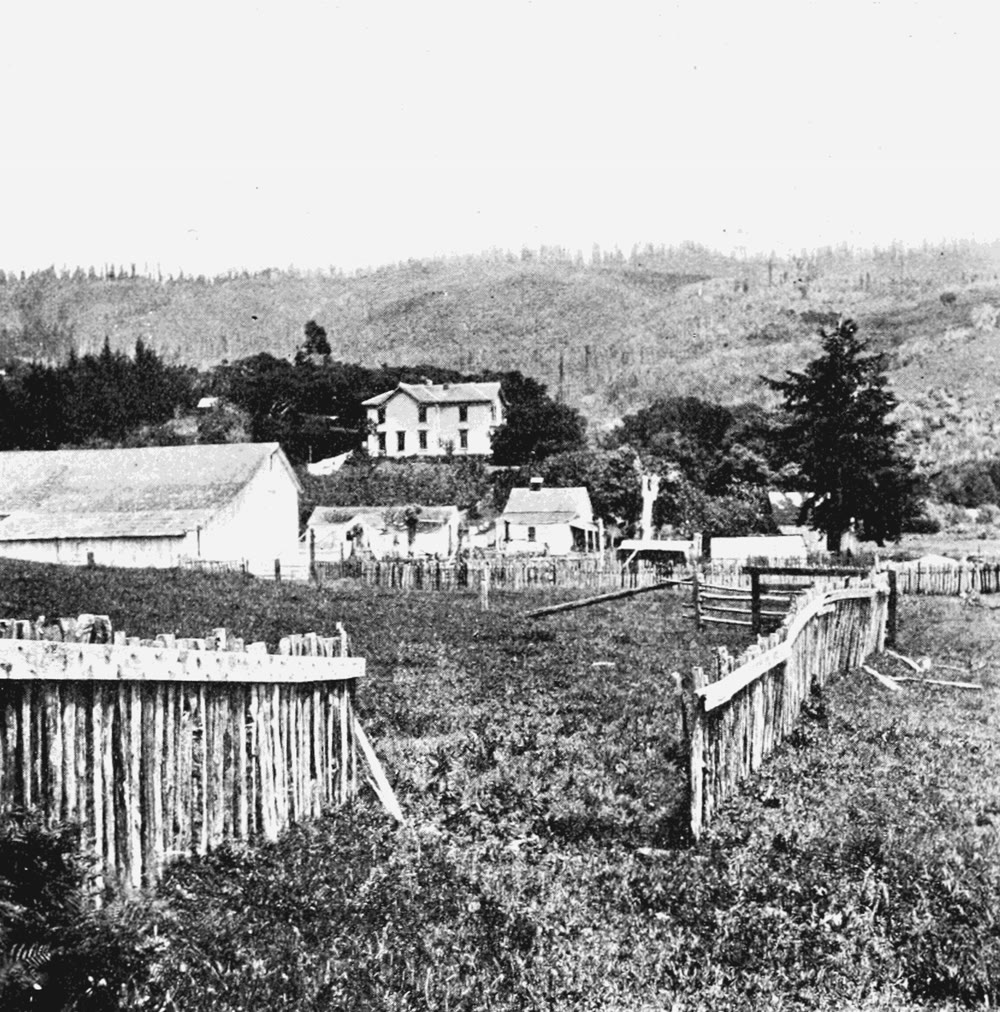
\includegraphics[height=5.6cm]{images/book3/b1-fence-1906.jpg}\hfill
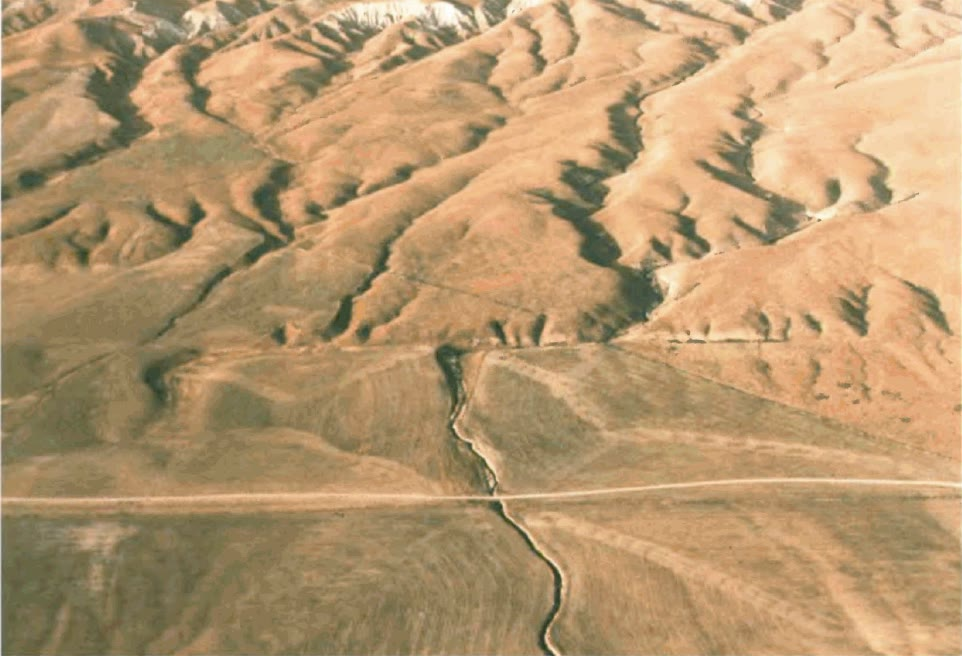
\includegraphics[height=5.6cm]{images/book3/b1-wallace-creek.jpg}
\par\smallskip{\small À gauche~: des clôtures dans des terres cultivées du comté de Marin, au nord de San
Francisco, traversées par la rupture de 1906, publiées la même année comme «~terre
séparée par la faille du séisme~». Photographie tirée de \emph{Popular Science
Monthly}, vol.~69 (1906), domaine public. À droite~: Wallace Creek, plaine de Carrizo,
vu du ciel~: le cours d'eau descend des collines (en haut), et là où il
traverse la faille de San Andreas, au pied des collines, son chenal fait un décrochement
de \qty{130}{m}, le décalage accumulé en des milliers d'années de
séismes. Photographie~:
R.~E.~Wallace, U.S. Geological Survey, domaine public. Les deux proviennent de Wikimedia
Commons.}
\label{fig:b1:earthquake-source:offsets}
\end{omfigure}
% ledger: commons:psm-fence, commons:wallace-creek

La proposition donne une moyenne, non un horaire. Près de Parkfield, sur la
même faille, un séisme de magnitude environ 6 en 1857 a été suivi de cinq
autres, très semblables, sur le même tronçon d'environ \qty{30}{km}, à des intervalles de
près de 22 ans jusqu'en 1966~; le suivant était attendu avant 1993, et est venu en
2004, avec une \omterm{def:b1:earthquake-source:mw}{magnitude de moment} de 6.0 et sans signe précurseur net. La
résistance d'une faille, le glissement de chaque séisme et le chargement par ses
voisines varient tous d'un cycle à l'autre, et le \omterm{def:b1:earthquake-source:seismic-cycle}{cycle sismique} est
mieux décrit par un \omterm{def:b1:earthquake-source:seismic-cycle}{intervalle de récurrence} moyen et une dispersion autour de lui que par
une période.
% ledger: pp1515:parkfield, bl85:parkfield, usgs:hist-mw, bakun:2005

Certains segments de faille ne se bloquent pas du tout. Entre Parkfield et San Juan
Bautista, la section centrale de la faille de San Andreas flue~: un glissement régulier sur
la faille absorbe presque tout le mouvement des plaques, et peu de déformation, voire aucune,
s'accumule de part et d'autre, si bien que cette section n'a pas de grands
séismes~; la grande rupture de 1857 a commencé à son extrémité sud et celle de
1906 s'est arrêtée à la nord. Une faille qui flue sur une partie de son aire n'est
bloquée qu'en partie, ce qui est le coefficient $c$ de la proposition.
% ledger: pp1515:creep, pp1515:1906

\begin{inthefield}[Lire d'anciens séismes dans une tranchée]
Les instruments enregistrent les séismes depuis un peu plus d'un siècle, bien
moins qu'un cycle de la plupart des failles. Les paléosismologues allongent l'enregistrement en
lisant le sol. On creuse une tranchée de quelques mètres de profondeur à travers une faille active
là où des couches de sédiments se sont déposées de façon continue, dans un marais, un lac
ou un petit cône alluvial. Sur ses parois, chaque séisme se montre sous forme de couches coupées et
décalées par la faille et recouvertes, intactes, par de plus jeunes~; d'un escarpement enfoui
par des dépôts ultérieurs~; de sable qui s'est liquéfié et est monté par des fissures pour s'étaler
sur la surface de l'époque. La tourbe ou les restes de plantes dans les couches juste en dessous
et juste au-dessus de chaque cassure sont datés par le radiocarbone, et encadrent ainsi la date de
chaque séisme~: un marais sur la faille de San Andreas garde l'enregistrement de douze.
Le long des côtes, des nappes de sable déposées par des tsunamis et des marais qui se sont affaissés
brusquement d'un mètre environ, enfouis sous la vase de marée, enregistrent les grands
séismes de subduction. Sur la faille de San Andreas, la plus grande part du glissement des temps historiques
est venue avec des séismes de magnitude 6 ou plus.
\end{inthefield}
% ledger: pp1515:pallett, atwater:1987

\begin{history}[Harry Fielding Reid et le rebond élastique]
Harry Fielding Reid, physicien américain, était membre de la commission d'État
qui étudia le séisme de 1906. En comparant les positions de
points levés en 1851--1865, en 1874--1892 et après le séisme, il
trouva que des points éloignés des deux côtés de la faille de San Andreas s'étaient déplacés
d'environ \qty{3.2}{m} l'un par rapport à l'autre depuis le premier levé, un peu
plus de la moitié du glissement d'environ \qty{6}{m} sur la faille~: un demi-siècle avant
le séisme, la déformation qui allait rompre la faille était déjà à moitié constituée. Seules
des forces élastiques pouvaient avoir déplacé le sol si soudainement, et il appela ce
retour soudain le \omterm{def:b1:earthquake-source:seismic-cycle}{rebond élastique}. Il le publia dans le deuxième volume du rapport
de la commission, en 1910~; c'est toujours le principal modèle du
\omterm{def:b1:earthquake-source:seismic-cycle}{cycle sismique}. Le positionnement par satellite a depuis mesuré la courbure qu'il ne pouvait
qu'inférer.
\end{history}
% ledger: reid:1910, pp1515:1906

\section{Moment sismique et magnitude}\label{sec:b1:earthquake-source:moment}

La taille d'un séisme est la quantité de glissement qu'il a faite, sur l'aire de
faille qui a glissé, pondérée par la rigidité des roches.

\begin{definition}[Moment sismique]\label{def:b1:earthquake-source:moment}
Soit un séisme qui glisse de la quantité moyenne $D$ sur une rupture d'aire $A$,
dans des roches de module de cisaillement $\mu$ (la lettre désigne aussi un coefficient de frottement,
au \cref{ch:b1:stress-strain-rheology}~; le contexte dit lequel). Son \emph{moment sismique}\index{moment sismique} est
\[
  M_0 = \mu A D ,
\]
en newtons mètres.
\end{definition}
% ledger: usgs:gloss-moment

L'unité est celle d'un couple. Un glissement sur une faille émet les mêmes ondes que deux
paires de forces opposées, deux couples, appliquées au foyer, et le \omterm{def:b1:earthquake-source:moment}{moment
sismique} est le moment de chaque couple (cette équivalence, le double couple, est
démontrée dans le volume de troisième année). Le moment a les dimensions d'une énergie, mais
ce n'en est pas une~: l'énergie rayonnée sous forme d'ondes en est une petite fraction. Pour les
roches de la \omterm{def:b1:layered-earth:layers}{croûte}, on prend $\mu$ égal à \qty{30}{GPa}.
% ledger: kanamori:1977, sk:mu-locking

Le moment se calcule aujourd'hui à partir des ondes de longue période enregistrées dans le
monde entier. Pour le séisme du Tohoku du 11 mars 2011, la solution préférée par
l'U.S. Geological Survey donne $M_0 = \qty{5.59e22}{N.m}$. La faille a glissé
sur une aire d'environ \qty{400}{km} de long et \qty{150}{km} de large~; la définition
donne alors le glissement moyen
\[
  D = \frac{M_0}{\mu A}
    = \frac{\num{5.59e22}}{\num{3e10}\times\num{4e5}\times\num{1.5e5}}
    \approx \qty{31}{m} ,
\]
et des modèles de la rupture trouvent jusqu'à \qtyrange{50}{60}{m} dans sa partie la plus
déplacée.
% ledger: usgs:tohoku-mt, usgs:tohoku-summary

La magnitude du livre~1 était calculée à partir de l'amplitude des ondes sur un
sismogramme. De telles magnitudes mesurent les ondes d'une période~; dès qu'une rupture est
bien plus longue que leur longueur d'onde, de quelques à une cinquantaine de kilomètres,
l'amplitude cesse de croître avec sa taille, et la magnitude sature. La
magnitude des ondes de volume sature près de 6.5, la magnitude des ondes de surface près de 8.3.
En 2011, la première alerte au tsunami pour le Tohoku reposait sur une magnitude de ce
genre, qui est insuffisante pour les séismes de magnitude 8 ou plus, et elle
a sous-estimé les ondes. Le moment ne sature pas, et la magnitude est
maintenant définie à partir de lui.
% ledger: kanamori:1977, usgs:magtypes, jma:warning

\begin{definition}[Magnitude de moment]\label{def:b1:earthquake-source:mw}
La \emph{magnitude de moment}\index{magnitude de moment} d'un séisme de
\omterm{def:b1:earthquake-source:moment}{moment sismique} $M_0$, en newtons mètres, est
\[
  M_w = \tfrac23\left(\log_{10} M_0 - 9.1\right) .
\]
\end{definition}
% ledger: usgs:magtypes

Thomas Hanks et Hiroo Kanamori ont défini l'échelle en 1979, avec la constante
9.05 à la place de 9.1, une différence de 0.03 sur $M_w$~; les constantes ont été choisies
pour s'accorder avec les anciennes magnitudes là où celles-ci ne saturent pas. La magnitude du
livre~1 est, pour les grands séismes, ce nombre~: pour le Tohoku,
$M_w = \tfrac23(\log_{10}\num{5.59e22} - 9.1) = \tfrac23(22.75 - 9.1) = 9.1$~;
le grand séisme du Chili de 1960 et le séisme de l'Alaska de 1964 ont des
\omterm{def:b1:earthquake-source:mw}{magnitudes de moment} de 9.5 et 9.2, des tailles que les anciennes magnitudes ne pouvaient pas
montrer.
% ledger: hk:1979, kanamori:1977, usgs:hist-mw, usgs:tohoku-mt

\begin{proposition}[Une unité de magnitude]\label{prop:b1:earthquake-source:moment-steps}
Le \omterm{def:b1:earthquake-source:moment}{moment sismique} est $M_0 = 10^{1.5 M_w + 9.1}$ newtons mètres. Une unité de
\omterm{def:b1:earthquake-source:mw}{magnitude de moment} le multiplie par $10^{1.5} \approx 31.6$, deux unités par
$1000$. Si l'énergie rayonnée est une fraction fixe du moment, elle croît dans
le même rapport.
\end{proposition}

\begin{proof}
En résolvant la définition pour $M_0$ on obtient $\log_{10} M_0 = 1.5 M_w + 9.1$,
et pour deux séismes
\[
  \log_{10}\frac{M_0'}{M_0} = 1.5\,(M_w' - M_w) ,
\]
ce qui vaut $1.5$ pour une unité et $3$ pour deux. Si l'énergie rayonnée est $E_s = k M_0$ avec le même $k$
pour les deux, $E_s'/E_s = M_0'/M_0$.
\end{proof}

L'approximation de Kanamori, $E_s \approx M_0/(2\times10^4)$ (admise), est
l'hypothèse de la dernière phrase~; le facteur d'environ 32 en énergie par unité de
magnitude, rencontré au livre~1, est cette proposition. Comme $M_0 = \mu A D$ et que le
glissement d'un séisme croît avec la taille de sa rupture, une grande magnitude
demande une grande faille. La rupture de 1906, d'environ \qty{430}{km} de long, a brisé la
\omterm{def:b1:stress-strain-rheology:strength-envelope}{couche sismogène} jusqu'à environ \qty{15}{km} avec un glissement moyen de quelques mètres~:
avec $D = \qty{4}{m}$, $M_0 = \num{3e10}\times\num{4.3e5}\times\num{1.5e4}
\times 4 = \qty{7.7e20}{N.m}$ et $M_w = 7.9$, la magnitude du catalogue.
Une magnitude de 9 demande une rupture de centaines de kilomètres de long et de
plus d'une centaine de large, ce que seules les interfaces faiblement inclinées des
zones de subduction offrent.
% ledger: kanamori:1977, pp1515:1906, usgs:hist-mw, usgs:pp1515-thatcher

\section{Mécanismes au foyer}\label{sec:b1:earthquake-source:focal}

L'onde P est la première à atteindre un sismomètre. Son \omterm{def:b1:earthquake-source:focal-mechanism}{premier mouvement}, la première
oscillation de l'enregistrement vertical, est vers le haut là où l'onde arrive comme une poussée, le
sol comprimé et projeté loin de la source, et vers le bas là où elle arrive
comme une traction. Autour d'un séisme, poussées et tractions s'agencent selon un motif
qui donne l'orientation de la faille et la direction du glissement.

\begin{proposition}[Le signe du premier mouvement]\label{prop:b1:earthquake-source:first-motion}
Soit une faille de normale vers le haut $\mathbf n$ qui glisse du vecteur unitaire $\mathbf d$
(le glissement du \omterm{def:b1:faults-folds-fabrics:fault-elements}{compartiment supérieur} par rapport au \omterm{def:b1:faults-folds-fabrics:fault-elements}{compartiment inférieur}). L'onde P qui quitte
le foyer dans la direction unitaire $\mathbf x$ arrive comme une poussée si
$(\mathbf n\cdot\mathbf x)(\mathbf d\cdot\mathbf x) > 0$ et comme une traction si
$(\mathbf n\cdot\mathbf x)(\mathbf d\cdot\mathbf x) < 0$. Les poussées et les
tractions remplissent donc quatre quadrants, séparés par le plan de faille
($\mathbf n\cdot\mathbf x = 0$) et par le plan perpendiculaire au glissement
($\mathbf d\cdot\mathbf x = 0$).
\end{proposition}

\begin{proof}
Une direction avec $\mathbf n\cdot\mathbf x > 0$ pointe dans le \omterm{def:b1:faults-folds-fabrics:fault-elements}{compartiment supérieur},
qui se déplace de $\mathbf d$ par rapport au \omterm{def:b1:faults-folds-fabrics:fault-elements}{compartiment inférieur}~: la roche devant lui,
où $\mathbf d\cdot\mathbf x > 0$, est comprimée, et la roche derrière lui,
où $\mathbf d\cdot\mathbf x < 0$, est tirée. Une direction avec
$\mathbf n\cdot\mathbf x < 0$ pointe dans le \omterm{def:b1:faults-folds-fabrics:fault-elements}{compartiment inférieur}, qui se déplace de
$-\mathbf d$ par rapport au \omterm{def:b1:faults-folds-fabrics:fault-elements}{compartiment supérieur}, donc les signes sont inversés. Dans chaque
cas le \omterm{def:b1:earthquake-source:focal-mechanism}{premier mouvement} a le signe de $(\mathbf n\cdot\mathbf x)(\mathbf
d\cdot\mathbf x)$.
\end{proof}

L'argument ne donne que le signe. L'amplitude du \omterm{def:b1:earthquake-source:focal-mechanism}{premier mouvement}, qui est
proportionnelle à $2(\mathbf n\cdot\mathbf x)(\mathbf d\cdot\mathbf x)$ et donc
maximale à \ang{45} des deux plans et nulle sur eux, est admise ici
(volume de troisième année).

\begin{omfigure}
\begin{tikzpicture}[>={Stealth[length=5pt]}, font=\small, scale=0.95]
% map view around a vertical dextral fault striking north, the focus at the origin, rays leaving
% horizontally: pushes where (n.x)(d.x) > 0, i.e. in the NW and SE quadrants (beachballs.py,
% first_motion(0, 90, 180, x)). Stations at 20 azimuths on a circle of radius 2.3.
\fill[omThm!22] (0,0) -- (0,2.8) arc[start angle=90, end angle=180, radius=2.8] -- cycle;
\fill[omThm!22] (0,0) -- (0,-2.8) arc[start angle=270, end angle=360, radius=2.8] -- cycle;
\draw[black!40, line width=0.4pt] (0,0) circle[radius=2.8];
\draw[fault, line width=1.3pt] (0,-3.1) -- (0,3.1) node[above, font=\scriptsize] {faille (plan nodal)};
\draw[black, dashed, line width=0.7pt] (-3.1,0) -- (3.1,0) node[right, font=\scriptsize, align=left] {plan\\ auxiliaire};
% slip: the west block moves north, the east block south
\draw[->, line width=1pt] (-0.3,-0.8) -- (-0.3,0.8);
\draw[->, line width=1pt] (0.3,0.8) -- (0.3,-0.8);
% stations
\foreach \a in {9,27,...,351} {
  \pgfmathsetmacro{\fm}{-sin(\a)*cos(\a)}  % (n.x)(d.x) with n = east, d = south, x = (sin a, cos a)
  \pgfmathparse{\fm>0 ? 1 : 0}
  \ifnum\pgfmathresult=1
    \fill[black] ({2.3*sin(\a)},{2.3*cos(\a)}) circle[radius=0.11];
  \else
    \draw[black, fill=white, line width=0.6pt] ({2.3*sin(\a)},{2.3*cos(\a)}) circle[radius=0.11];
  \fi
}
% P and T axes
\draw[<-, omProp, line width=1.1pt] ({0.7*sin(45)},{0.7*cos(45)}) -- ({1.6*sin(45)},{1.6*cos(45)}) node[above right, font=\scriptsize, inner sep=1pt] {P};
\draw[<-, omProp, line width=1.1pt] ({0.7*sin(225)},{0.7*cos(225)}) -- ({1.6*sin(225)},{1.6*cos(225)});
\draw[->, omProp, line width=1.1pt] ({0.7*sin(315)},{0.7*cos(315)}) -- ({1.6*sin(315)},{1.6*cos(315)}) node[above left, font=\scriptsize, inner sep=1pt] {T};
\draw[->, omProp, line width=1.1pt] ({0.7*sin(135)},{0.7*cos(135)}) -- ({1.6*sin(135)},{1.6*cos(135)});
\fill (0,0) circle[radius=0.06];
% legend
\begin{scope}[xshift=4.6cm, yshift=2.4cm]
  \fill[black] (0,0) circle[radius=0.11]; \node[anchor=west, font=\scriptsize] at (0.2,0) {poussée~: premier mouvement vers le haut};
  \draw[black, fill=white, line width=0.6pt] (0,-0.5) circle[radius=0.11]; \node[anchor=west, font=\scriptsize] at (0.2,-0.5) {traction~: premier mouvement vers le bas};
  \fill[omThm!22] (-0.12,-1.12) rectangle (0.12,-0.88); \node[anchor=west, font=\scriptsize] at (0.2,-1.0) {quadrant en compression};
  \draw[->] (-0.1,-1.6) -- (-0.1,-1.25); \node[anchor=west, font=\scriptsize] at (0.2,-1.42) {N};
\end{scope}
\end{tikzpicture}
\par\smallskip{\small \omterm{def:b1:earthquake-source:focal-mechanism}{Premiers mouvements} autour d'une faille \omterm{def:b1:faults-folds-fabrics:fault-types}{dextre} verticale de direction
nord, vue de dessus, pour des ondes quittant le foyer horizontalement vers des
stations tout autour. Flèches noires~: le glissement des deux blocs. Les poussées
remplissent les quadrants nord-ouest et sud-est, les tractions les deux autres~; la
faille et le \omterm{def:b1:earthquake-source:focal-mechanism}{plan auxiliaire} les séparent. L'\omterm{def:b1:earthquake-source:focal-mechanism}{axe P} (flèches pointant vers l'intérieur)
bissecte les quadrants de traction, l'\omterm{def:b1:earthquake-source:focal-mechanism}{axe T} (flèches pointant vers l'extérieur) les quadrants de
poussée. Un glissement \omterm{def:b1:faults-folds-fabrics:fault-types}{senestre} sur le plan en tirets, le bloc au sud de lui
se déplaçant vers l'est, donnerait exactement le même motif
(\cref{prop:b1:earthquake-source:auxiliary}).}
\label{fig:b1:earthquake-source:quadrants}
\end{omfigure}

Le produit $(\mathbf n\cdot\mathbf x)(\mathbf d\cdot\mathbf x)$ ne change pas
quand on échange $\mathbf n$ et $\mathbf d$. Cette symétrie est le fait central
des \omterm{def:b1:earthquake-source:focal-mechanism}{mécanismes au foyer}.

\begin{definition}[Mécanisme au foyer, plan nodal, plan auxiliaire, axe P, axe T]\label{def:b1:earthquake-source:focal-mechanism}
Le \emph{premier mouvement}\index{premier mouvement} d'une onde P à un sismomètre est la
direction, vers le haut ou vers le bas, du premier mouvement du sol sur l'enregistrement
vertical. Le \emph{mécanisme au foyer}\index{mecanisme au foyer@mécanisme au foyer} d'un séisme est
l'orientation du plan de faille et la direction du glissement sur lui, telles que trouvées
à partir de ses ondes sismiques. Les deux plans perpendiculaires passant par le foyer qui
séparent les poussées des tractions sont ses \emph{plans nodaux}\index{plan nodal}~;
l'un est le plan de faille, et l'autre, perpendiculaire au glissement, est
le \emph{plan auxiliaire}\index{plan auxiliaire}. L'\emph{axe
P}\index{axe P} et l'\emph{axe T}\index{axe T} sont les directions à
\ang{45} des deux plans nodaux au milieu des quadrants de traction et des quadrants de
poussée~:
\[
  \mathbf P = \frac{\mathbf n - \mathbf d}{\sqrt2}, \qquad
  \mathbf T = \frac{\mathbf n + \mathbf d}{\sqrt2} .
\]
\end{definition}
% ledger: yvo:beachball, usgs:gloss-moment

\begin{proposition}[Les deux plans nodaux]\label{prop:b1:earthquake-source:auxiliary}
Un glissement $\mathbf d$ sur le plan de normale $\mathbf n$ et un glissement $\mathbf n$ sur
le plan de normale $\mathbf d$ donnent les mêmes \omterm{def:b1:earthquake-source:focal-mechanism}{premiers mouvements} dans toutes les directions.
Les \omterm{def:b1:earthquake-source:focal-mechanism}{premiers mouvements} déterminent donc les deux \omterm{def:b1:earthquake-source:focal-mechanism}{plans nodaux}, les \omterm{def:b1:earthquake-source:focal-mechanism}{axes P} et T et
le sens du glissement sur chaque plan, mais ils ne disent pas quel \omterm{def:b1:earthquake-source:focal-mechanism}{plan nodal} est la
faille.
\end{proposition}

\begin{proof}
Le signe de $(\mathbf n\cdot\mathbf x)(\mathbf d\cdot\mathbf x)$ est inchangé
par l'échange de $\mathbf n$ et $\mathbf d$~; les plans
$\mathbf n\cdot\mathbf x = 0$ et $\mathbf d\cdot\mathbf x = 0$ sont échangés,
et $\mathbf n \pm \mathbf d$ sont inchangés. Un couple $(\mathbf n, \mathbf d)$ et
le couple $(-\mathbf n, -\mathbf d)$, qui décrit le même glissement vu de
l'autre bloc, donnent aussi le même produit. Rien dans les \omterm{def:b1:earthquake-source:focal-mechanism}{premiers mouvements}
ne distingue les deux descriptions.
\end{proof}

Pour décider quel \omterm{def:b1:earthquake-source:focal-mechanism}{plan nodal} a glissé, les sismologues utilisent d'autres indices~: le
plan le long duquel s'alignent les répliques, la faille vue en surface, la
limite de plaques sur laquelle se trouve le séisme. Pour le grand séisme de Sumatra--Andaman de
2004, les deux \omterm{def:b1:earthquake-source:focal-mechanism}{plans nodaux} plongent de \ang{8} vers le nord-est et de
\ang{83} vers le sud-ouest. Les séismes antérieurs de la région et les
modèles de plaques placent tous deux le \omterm{def:b1:active-margins:slab}{panneau plongeant} le long d'un plan plongeant doucement vers le
nord-est, et le plan peu profond est pris pour la faille~: le séisme a rompu
l'interface de plaques de la zone de subduction, et ses répliques se sont étendues sur
plus de \qty{1300}{km}.
% ledger: usgs:sumatra-mt, usgs:sumatra-summary

Comme l'\omterm{def:b1:earthquake-source:focal-mechanism}{axe P} se trouve au milieu des tractions et l'\omterm{def:b1:earthquake-source:focal-mechanism}{axe T} au milieu
des poussées, on les lit souvent comme les directions de plus forte et de plus faible
contrainte compressive, $\sigma_1$ et $\sigma_3$. Ils n'en sont que des approximations.
Une nouvelle faille se forme à $\ang{45} - \phi/2$ de $\sigma_1$, non à \ang{45}
(\cref{ch:b1:stress-strain-rheology}), et une ancienne faille peut glisser sous un angle encore
différent, si bien que les axes d'un séisme peuvent se trouver à des dizaines de degrés des
\omterm{def:b1:stress-strain-rheology:principal}{contraintes principales}~; les contraintes d'une région se trouvent à partir des mécanismes
de nombreux séismes ensemble.

Un \omterm{def:b1:earthquake-source:focal-mechanism}{mécanisme au foyer} vit sur une sphère autour du foyer. On le trace sur la moitié inférieure
de cette sphère, que traverse chaque rai vers une station lointaine, projetée
sur un disque~: un rai de vecteur unitaire $\mathbf x = (E, N, U)$, avec $U \le 0$, est
tracé en
\[
  (X, Y) = \frac{(E, N)}{\sqrt{1 - U}} ,
\]
la verticale au centre et l'horizontale sur le cercle unité. Cette
projection conserve les aires (admis~; les projections de la sphère sont étudiées dans
le volume de troisième année), si bien que chaque quadrant couvre sa vraie part du disque. Les
quadrants de poussée sont grisés~; l'image s'appelle un ballon de plage.
% ledger: yvo:beachball

\begin{omfigure}
\begin{tikzpicture}[font=\small]
% lower-hemisphere equal-area beach balls, compressional quadrants shaded (figdata/bachelor-1/beachballs.py)
\foreach \n/\c/\t/\x in {normal/2/{(a) faille normale\\ $090/60$, pitch \ang{-90}}/0,
                         reverse/1/{(b) faille inverse\\ $090/30$, pitch \ang{90}}/3.65,
                         strikeslip/2/{(c) faille décrochante\\ $090/90$, pitch \ang{180}}/7.3,
                         tohoku/2/{(d) Tohoku, 2011\\ $282/8$, pitch \ang{78}}/10.95} {
  \begin{axis}[at={(\x cm,0)}, anchor=center, width=2.9cm, height=2.9cm, scale only axis,
      axis equal image, xmin=-1.04, xmax=1.04, ymin=-1.04, ymax=1.04, hide axis, clip=false]
    \fill[white] (axis cs:0,0) circle[radius=1];
    \addplot[fill=omThm!55, draw=none] table[x=X, y=Y] {figdata/out/bachelor-1-beachballs-\n-c1.dat};
    \ifnum\c=2
      \addplot[fill=omThm!55, draw=none] table[x=X, y=Y] {figdata/out/bachelor-1-beachballs-\n-c2.dat};
    \fi
    \addplot[black, line width=0.6pt] table[x=X, y=Y] {figdata/out/bachelor-1-beachballs-\n-p1.dat};
    \addplot[black, line width=0.6pt] table[x=X, y=Y] {figdata/out/bachelor-1-beachballs-\n-p2.dat};
    \draw[black, line width=0.8pt] (axis cs:0,0) circle[radius=1];
    \draw[black, line width=0.5pt] (axis cs:0,1) -- (axis cs:0,1.12) node[above, font=\scriptsize, inner sep=1pt] {N};
    \addplot[only marks, mark=none, nodes near coords={\textbf{P}}, nodes near coords align=center, every node near coord/.append style={font=\scriptsize, inner sep=0pt}] table[x=X, y=Y] {figdata/out/bachelor-1-beachballs-\n-P.dat};
    \addplot[only marks, mark=none, nodes near coords={\textbf{T}}, nodes near coords align=center, every node near coord/.append style={font=\scriptsize, inner sep=0pt}] table[x=X, y=Y] {figdata/out/bachelor-1-beachballs-\n-T.dat};
    \node[anchor=north, align=center, font=\scriptsize] at (axis cs:0,-1.12) {\t};
  \end{axis}
}
\end{tikzpicture}
\par\smallskip{\small Ballons de plage~: l'hémisphère inférieur autour du foyer en
projection équivalente, nord en haut, les quadrants de poussée grisés, P et T marquant les
axes (une lettre est ramenée vers l'intérieur quand son axe est près du bord). Chaque mécanisme
est donné par l'\omterm{def:b1:geological-maps:attitude}{attitude} d'un \omterm{def:b1:earthquake-source:focal-mechanism}{plan nodal}, \omterm{def:b1:geological-maps:attitude}{sens du pendage} et \omterm{def:b1:geological-maps:attitude}{pendage}, et le \omterm{def:b1:faults-folds-fabrics:fault-elements}{pitch}
du glissement sur lui. (a) Une \omterm{def:b1:faults-folds-fabrics:fault-types}{faille normale} plongeant de \ang{60} vers l'est~: le quadrant de traction
remplit le centre. (b) Une \omterm{def:b1:faults-folds-fabrics:fault-types}{faille inverse} plongeant de \ang{30} vers l'est~: le quadrant de poussée
remplit le centre. (c) Une \omterm{def:b1:faults-folds-fabrics:fault-types}{faille décrochante} verticale~: quatre quadrants se rejoignant au
centre. (d) Le séisme du Tohoku de 2011 (tenseur des moments de l'U.S. Geological Survey)~: un
\omterm{def:b1:faults-folds-fabrics:fault-types}{chevauchement} sur un plan plongeant de \ang{8} vers $282$, sous le Japon, avec le
\omterm{def:b1:earthquake-source:focal-mechanism}{plan auxiliaire} raide à l'est.}
\label{fig:b1:earthquake-source:beachballs}
\end{omfigure}
% ledger: usgs:tohoku-mt

Les sismologues donnent un mécanisme par la direction, le \omterm{def:b1:geological-maps:attitude}{pendage} et le \omterm{def:b1:faults-folds-fabrics:fault-elements}{pitch} de chaque \omterm{def:b1:earthquake-source:focal-mechanism}{plan nodal}~;
la direction est le \omterm{def:b1:geological-maps:attitude}{sens du pendage} moins \ang{90}, comme au
\cref{ch:b1:faults-folds-fabrics}. Pour le Tohoku, les plans sont
$192/8/78$ et $24/81/91$ en direction, \omterm{def:b1:geological-maps:attitude}{pendage} et \omterm{def:b1:faults-folds-fabrics:fault-elements}{pitch}, et les \omterm{def:b1:earthquake-source:focal-mechanism}{axes P} et T ont pour direction
$113$ et $296$ et plongent de \ang{36} et \ang{53}. Le \omterm{def:b1:earthquake-source:focal-mechanism}{plan auxiliaire} se déduit
du plan de faille~: sa normale est $\mathbf d$ et son glissement est $\mathbf n$, de sorte
qu'on le trouve en calculant $\mathbf n$ et $\mathbf d$ à partir de la direction, du \omterm{def:b1:geological-maps:attitude}{pendage}
et du \omterm{def:b1:faults-folds-fabrics:fault-elements}{pitch}, en les échangeant, et en relisant la direction, le \omterm{def:b1:geological-maps:attitude}{pendage} et le \omterm{def:b1:faults-folds-fabrics:fault-elements}{pitch}
(exercice~\ref{exo:b1:earthquake-source:7}).
% ledger: usgs:tohoku-mt

\begin{method}[Lire un ballon de plage]\label{met:b1:earthquake-source:beachball}
\begin{enumerate}
  \item Regarder le centre, qui est la verticale. Grisé (une poussée droit
        vers le bas)~: une composante inverse ou de \omterm{def:b1:faults-folds-fabrics:fault-types}{chevauchement}~; blanc~: une composante normale. Deux
        diamètres droits se croisant au centre~: un mécanisme décrochant.
  \item Trouver les deux \omterm{def:b1:earthquake-source:focal-mechanism}{plans nodaux}, les courbes qui bordent les quadrants. Un
        plan passant par le centre est vertical~; un plan plonge vers le côté du
        centre où se trouve sa courbe, d'autant plus doucement que la courbe
        est proche du bord.
  \item Trouver l'\omterm{def:b1:earthquake-source:focal-mechanism}{axe T} au milieu des quadrants grisés et l'\omterm{def:b1:earthquake-source:focal-mechanism}{axe P} au milieu
        des blancs~: le sol a été raccourci selon P et
        allongé selon T.
  \item Pour chaque \omterm{def:b1:earthquake-source:focal-mechanism}{plan nodal}, lire ou calculer le \omterm{def:b1:faults-folds-fabrics:fault-elements}{pitch}, et nommer la faille qu'il
        serait avec la \cref{def:b1:faults-folds-fabrics:fault-types}. Les deux
        plans partagent toujours le sens en \omterm{def:b1:geological-maps:attitude}{pendage}, normal ou inverse, et ont
        des sens en direction opposés~: un mécanisme décrochant donne un plan \omterm{def:b1:faults-folds-fabrics:fault-types}{dextre}
        et un plan \omterm{def:b1:faults-folds-fabrics:fault-types}{senestre}.
  \item Choisir le plan de faille d'après les répliques, la géologie ou la limite
        de plaques.
\end{enumerate}
\end{method}

\begin{inthelab}[Dans un observatoire sismologique]
\begin{minipage}[t]{0.6\linewidth}\vspace{0pt}
Quelques minutes après un grand séisme, ses ondes ont été enregistrées par des centaines
de stations, et les données parviennent aux analystes des observatoires en temps quasi
réel. Les premières arrivées de l'onde P, qui atteignent les stations d'autant plus tard
qu'elles sont éloignées, sont pointées sur les enregistrements pour localiser le foyer. Puis les ondes longues
et lentes enregistrées pendant les dizaines de minutes suivantes sont comparées à des ondes
calculées pour des sources d'essai~; la source dont les ondes s'ajustent le mieux donne le tenseur des moments,
qui contient ensemble le \omterm{def:b1:earthquake-source:moment}{moment sismique}, la \omterm{def:b1:earthquake-source:mw}{magnitude de moment} et les deux
\omterm{def:b1:earthquake-source:focal-mechanism}{plans nodaux}. Pour les petits séismes, trop faibles pour cela, les analystes
lisent les \omterm{def:b1:earthquake-source:focal-mechanism}{premiers mouvements} sur les enregistrements les plus proches et leur ajustent les \omterm{def:b1:earthquake-source:focal-mechanism}{plans nodaux},
de la façon décrite dans cette section. Chaque solution est publiée avec ses
incertitudes, et révisée à mesure que d'autres données arrivent.
\end{minipage}\hfill
\begin{minipage}[t]{0.36\linewidth}\vspace{0pt}
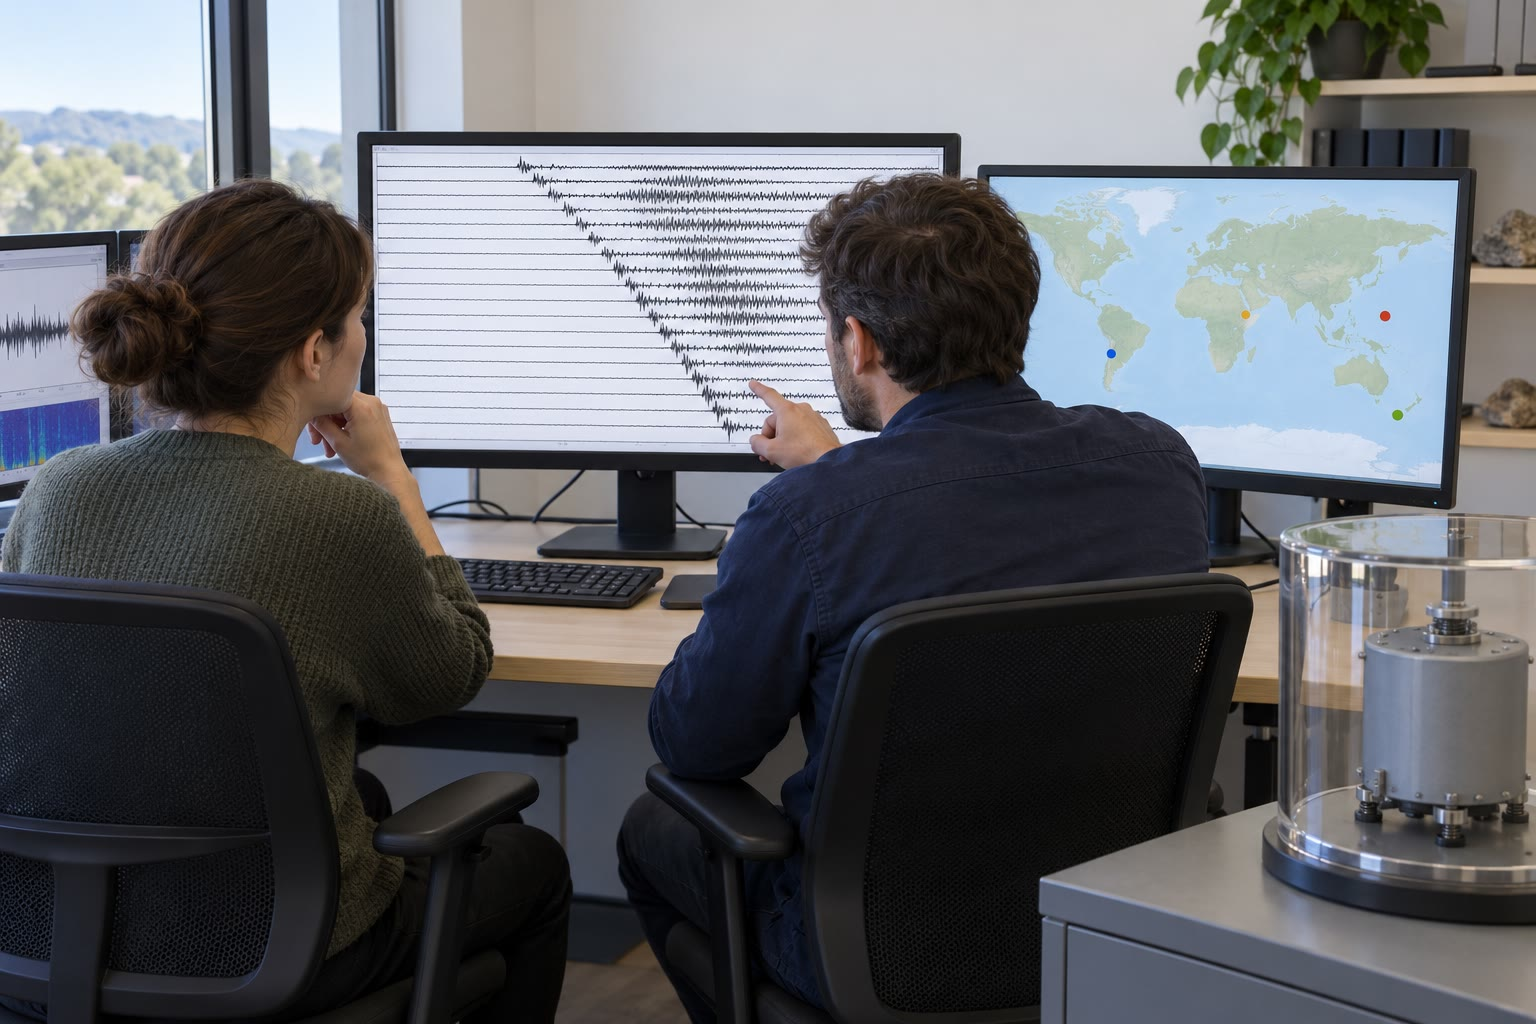
\includegraphics[width=\linewidth]{images/book3/ai/b1-seismic-analysis.jpg}

{\scriptsize Des sismologues lisant une section d'enregistrements, les traces d'un même
séisme à des stations classées par distance (illustration IA).}
\end{minipage}
\end{inthelab}
% ledger: yvo:beachball

\section{Mesurer le chargement~: la géodésie}\label{sec:b1:earthquake-source:geodesy}

Entre les séismes, une faille bloquée est invisible aux sismomètres, mais le
sol autour d'elle bouge. Des stations permanentes de positionnement par satellite mesurent ce
mouvement, et la façon dont leurs vitesses changent à travers une faille dit jusqu'à quelle profondeur elle
est bloquée.

\begin{definition}[Profondeur de blocage]\label{def:b1:earthquake-source:locking-depth}
La \emph{profondeur de blocage}\index{profondeur de blocage} d'une faille est la profondeur jusqu'à
laquelle elle est bloquée entre les séismes, la faille en dessous glissant régulièrement à la
vitesse à long terme~; c'est la profondeur de la partie de la faille qui glisse lors du prochain
séisme.
\end{definition}
% ledger: usgs:pp1515-thatcher

\begin{proposition}[Vitesse intersismique à travers une faille décrochante]\label{prop:b1:earthquake-source:interseismic}
Soit une \omterm{def:b1:faults-folds-fabrics:fault-types}{faille décrochante} verticale dans un demi-espace élastique, bloquée de la
surface à la profondeur $D$, et glissant à la vitesse $V$ en dessous. La vitesse de
la surface parallèlement à la faille, à la distance $x$ d'elle, est
\[
  v(x) = \frac{V}{\pi}\arctan\frac{x}{D} .
\]
Si la faille glisse ensuite de $s$ de la surface à la profondeur $D$ lors d'un
séisme, la surface se déplace de $u(x) = (s/\pi)\arctan(D/x)$ pour $x > 0$, et de
$-u(-x)$ pour $x < 0$.
\end{proposition}
\admitted

Ce modèle, dû à Savage et Burford, est la forme la plus simple du \omterm{def:b1:earthquake-source:seismic-cycle}{rebond
élastique}, et la courbe de la clôture de la première figure. Ses propriétés découlent
de la formule.

\begin{proposition}[Lire le profil intersismique]\label{prop:b1:earthquake-source:profile}
Dans le modèle de la \cref{prop:b1:earthquake-source:interseismic}~:
\begin{enumerate}[label=(\alph*)]
  \item loin de la faille la vitesse tend vers $\pm V/2$, les deux plaques
        se déplaçant à $V$ l'une par rapport à l'autre~;
  \item la moitié du changement de vitesse à travers la faille se produit dans la
        distance $D$ d'elle~: $v(\pm D) = \pm V/4$~;
  \item la vitesse de déformation en cisaillement de la surface, $\mathrm dv/\mathrm dx$, est
        maximale sur la faille, où elle vaut $V/(\pi D)$~;
  \item si la faille, après un chargement pendant le temps $t$, glisse de $s = Vt$ lors d'un
        séisme, le sol se retrouve déplacé de $\pm s/2$ partout de
        chaque côté~: le cycle ne laisse aucune courbure permanente, seulement le décalage $s$
        sur la faille.
\end{enumerate}
\end{proposition}

\begin{proof}
(a) $\arctan(x/D) \to \pm\pi/2$ quand $x \to \pm\infty$. (b) $\arctan 1 = \pi/4$,
donc $v(D) = V/4$, et $v$ est impaire. (c) $\mathrm dv/\mathrm dx = (V/\pi D)/(1 +
x^2/D^2)$, maximale en $x = 0$. (d) Pour $x > 0$, le chargement a déplacé le
sol de $t\,v(x) = (s/\pi)\arctan(x/D)$ et le séisme de
$(s/\pi)\arctan(D/x)$~; puisque $\arctan y + \arctan(1/y) = \pi/2$ pour $y > 0$,
la somme est $s/2$. La même chose vaut avec les signes inversés pour $x < 0$.
\end{proof}

La propriété (b) donne la \omterm{def:b1:earthquake-source:locking-depth}{profondeur de blocage} à partir d'un profil de stations~: c'est la
distance à la faille à laquelle la vitesse a changé d'un quart de $V$
par rapport à sa valeur sur la faille. Un blocage peu profond concentre la déformation près de la
faille (figure ci-dessous), un blocage profond l'étale sur une large ceinture. Le long du système de
San Andreas, les \omterm{def:b1:earthquake-source:locking-depth}{profondeurs de blocage} trouvées par la géodésie vont de presque 0, sur les
segments qui fluent, à \qty{26}{km}, et s'accordent avec les profondeurs des
séismes~: la partie bloquée est la \omterm{def:b1:stress-strain-rheology:strength-envelope}{couche sismogène} du
\cref{ch:b1:stress-strain-rheology}. Pour une vitesse de glissement de
\qty{34}{mm.an^{-1}} et une \omterm{def:b1:earthquake-source:locking-depth}{profondeur de blocage} de \qty{15}{km}, la vitesse de déformation en cisaillement
sur la faille est $\num{0.034}/(\pi\times\num{15000}) = \num{7.2e-7}$ par an,
ce qui courbe une ligne à travers la faille de moins d'un millimètre par kilomètre en
un an, et pourtant stocke, en deux siècles, les plusieurs mètres de glissement d'un grand
séisme.
% ledger: sk:mu-locking, usgs:pp1515-wallace, usgs:pp1515-thatcher

\begin{omfigure}
\begin{tikzpicture}[font=\small]
\begin{axis}[omrecord, width=11cm, height=5.6cm, xmin=-100, xmax=100, ymin=-19, ymax=19,
    xlabel={distance à la faille $x$ (km)}, ylabel={vitesse $v$ (\unit{mm.an^{-1}})},
    legend style={font=\scriptsize, at={(0.02,0.96)}, anchor=north west}, legend cell align=left]
  \addplot[omDef, line width=0.9pt, dashed] table[x=x, y=v5] {figdata/out/bachelor-1-interseismic-profiles.dat};
  \addplot[omThm, line width=1.1pt] table[x=x, y=v15] {figdata/out/bachelor-1-interseismic-profiles.dat};
  \addplot[omProp, line width=0.9pt, dotted] table[x=x, y=v25] {figdata/out/bachelor-1-interseismic-profiles.dat};
  \legend{$D = \qty{5}{km}$, $D = \qty{15}{km}$, $D = \qty{25}{km}$}
  \draw[black!50, dashed] (axis cs:-100,17) -- (axis cs:100,17);
  \draw[black!50, dashed] (axis cs:-100,-17) -- (axis cs:100,-17);
  \node[anchor=north west, font=\scriptsize] at (axis cs:-30,17) {$+V/2$};
  \node[anchor=south west, font=\scriptsize] at (axis cs:30,-17) {$-V/2$};
  \draw[black!60] (axis cs:0,-19) -- (axis cs:0,19);
  \node[anchor=east, font=\scriptsize] at (axis cs:-1,5) {faille};
\end{axis}
\end{tikzpicture}
\par\smallskip{\small Vitesse du sol parallèlement à une \omterm{def:b1:faults-folds-fabrics:fault-types}{faille décrochante} bloquée,
par rapport à la trace de la faille, pour une vitesse de glissement $V = \qty{34}{mm.\year^{-1}}$,
celle de la faille de San Andreas à Wallace Creek, et trois \omterm{def:b1:earthquake-source:locking-depth}{profondeurs de blocage}
(\cref{prop:b1:earthquake-source:interseismic}). Plus le blocage est peu profond, plus la
ceinture où la vitesse change est étroite.}
\label{fig:b1:earthquake-source:interseismic}
\end{omfigure}
% ledger: usgs:pp1515-wallace

Le positionnement par satellite mesure le sol en quelques stations. Les satellites radar
le mesurent partout~: deux images radar de la même zone prises depuis la même
orbite à des moments différents sont comparées onde par onde, et la différence de
phase cartographie le changement de la distance entre le sol et le satellite,
point par point, à cent mètres d'écart, sans réseau de stations installé à
l'avance. La première carte de ce genre, d'un grand séisme californien de 1992, montra
son déplacement cosismique en une seule image et s'accorda avec le glissement
mesuré sur le terrain et par arpentage~; la technique, l'interférométrie radar,
relève du volume de troisième année.
% ledger: massonnet:1993

\section{À quelle fréquence~: la loi de Gutenberg--Richter}\label{sec:b1:earthquake-source:gr}

Les petits séismes sont bien plus fréquents que les grands, et d'une façon
remarquablement régulière.

\begin{proposition}[Loi de Gutenberg--Richter]\label{prop:b1:earthquake-source:gutenberg-richter}
Dans une région et sur une période\index{loi de Gutenberg--Richter}, le nombre $N$ de séismes de magnitude au moins
$M$ obéit à
\[
  \log_{10} N = a - bM ,
\]
pour tout $M$ au-dessus de la \omterm{def:b1:earthquake-source:b-value}{magnitude de complétude} du catalogue, avec des
constantes $a$ et $b$ qui dépendent de la région~; $b$ est proche de 1 dans la plupart des
régions actives.
\end{proposition}
\admitted
% ledger: fd:1993, gr:1944

La loi est un résultat d'observation, publié par Beno Gutenberg et Charles
Richter pour la Californie en 1944 et trouvé depuis partout~; aucune théorie ne
la dérive encore, ni la valeur de $b$.
% ledger: gr:1944

\begin{definition}[Valeur b, magnitude de complétude]\label{def:b1:earthquake-source:b-value}
La constante $b$ de la \omterm{prop:b1:earthquake-source:gutenberg-richter}{loi de Gutenberg--Richter} d'une région est sa
\emph{valeur b}\index{valeur b}. La \emph{magnitude de
complétude}\index{magnitude de completude@magnitude de complétude} d'un catalogue est la plus petite
magnitude au-dessus de laquelle il enregistre tous les séismes de la région et de la période.
\end{definition}

Une \omterm{def:b1:earthquake-source:b-value}{valeur b} de 1 signifie dix fois moins de séismes à chaque unité de magnitude.
Sous la \omterm{def:b1:earthquake-source:b-value}{magnitude de complétude}, les décomptes sont inférieurs à la droite, parce que
les petits séismes sont enregistrés par trop peu de stations pour être localisés~: la loi
semble se courber, et $b$ doit être mesuré au-dessus d'elle. Pour la Terre entière,
divisée en séismes superficiels, intermédiaires et profonds, les valeurs mesurées
se situent entre 0.72 et 1.34, mais elles diffèrent de \qty{30}{\percent} ou plus d'un
catalogue, d'un intervalle de magnitudes ou d'une méthode à l'autre~: une valeur loin de 1 est
d'abord une raison de vérifier le catalogue.
% ledger: fd:1993

\begin{omfigure}
\begin{tikzpicture}[font=\small]
\begin{axis}[omrecord, width=6.4cm, height=5.8cm, ymode=log, xmin=5.8, xmax=9.3, ymin=0.01, ymax=300,
    xlabel={magnitude $M$}, ylabel={événements de magnitude $\ge M$ par an},
    log basis y=10, title={(a) fréquence et magnitude}, title style={font=\small}]
  \addplot[omProp, line width=0.9pt, domain=5.8:9.3] table[x=M, y=rate] {figdata/out/bachelor-1-gutenberg_richter-fit.dat};
  \addplot[only marks, mark=*, mark size=1.3pt, omDef] table[x=M, y=rate] {figdata/out/bachelor-1-gutenberg_richter-counts.dat};
  \draw[black!50, dashed] (axis cs:7.5,0.01) -- (axis cs:7.5,300);
  \node[anchor=south west, font=\scriptsize, omProp] at (axis cs:8.45,0.5) {$b = 1.01$};
  \node[anchor=north west, font=\scriptsize, align=left] at (axis cs:7.55,200) {ajustée sur\\ $6.0 \le M \le 7.5$};
\end{axis}
\begin{axis}[omrecord, at={(7.6cm,0)}, width=6.4cm, height=5.8cm, xmin=5.8, xmax=9.3, ymin=0, ymax=1.05,
    xlabel={magnitude $M$}, ylabel={part du moment des événements $\ge M$},
    title={(b) où va le moment}, title style={font=\small}]
  \addplot[const plot, omDef, line width=0.9pt] table[x=M, y=share] {figdata/out/bachelor-1-gutenberg_richter-moment.dat};
\end{axis}
\end{tikzpicture}
\par\smallskip{\small Les \num{7031} séismes de magnitude 6 ou plus dans le
monde, 1976--2025 (catalogue de l'U.S. Geological Survey). (a) Le nombre annuel de
séismes de magnitude au moins $M$~; la droite est l'ajustement des moindres carrés de
$\log_{10} N$ en fonction de $M$ de 6.0 à 7.5, où chaque décompte dépasse 200~:
$\log_{10} N = 8.20 - 1.01\,M$ par an. Au-dessus de la magnitude 8 les quelques événements tombent
sous la droite. (b) La part du \omterm{def:b1:earthquake-source:moment}{moment sismique} total libéré par les
séismes de magnitude au moins $M$, chaque moment calculé comme
$10^{1.5M + 9.1}$\,\unit{N.m}~: les 40 séismes de magnitude 8 ou plus
en ont libéré \qty{63}{\percent}.}
\label{fig:b1:earthquake-source:gutenberg-richter}
\end{omfigure}
% ledger: data:usgs-comcat (fit and shares computed in figdata/bachelor-1/gutenberg_richter.py)

Pour le catalogue mondial de la figure, la loi avec $a = 8.20$ et $b = 1.01$
prédit 14 séismes de magnitude 7 ou plus par an, comme observé, et 1.35 de
magnitude 8 ou plus, alors que 40 en cinquante ans, 0.8 par an, ont été enregistrés. Que
les plus grands séismes soient vraiment moins nombreux que la droite, comme la taille finie des
failles le suggérerait, ou seulement assez rares pour manquer sur cinquante ans, n'est pas
tranché par si peu d'événements. Environ une magnitude sur neuf de ce catalogue est une
magnitude d'ondes de surface ou de volume, qui saturent~; les plus grands événements
ont tous des \omterm{def:b1:earthquake-source:mw}{magnitudes de moment}.
% ledger: data:usgs-comcat

Les nombreux petits séismes font peu du travail. Leur nombre est multiplié par dix
à chaque unité de magnitude en moins, mais leurs moments sont divisés par 31.6.

\begin{proposition}[Les plus grands séismes libèrent l'essentiel du moment]\label{prop:b1:earthquake-source:largest}
Soient des séismes qui obéissent à la \omterm{prop:b1:earthquake-source:gutenberg-richter}{loi de Gutenberg--Richter} avec $b < 1.5$, jusqu'à une
plus grande magnitude $M_{\max}$, et groupés en classes larges d'une unité de
magnitude, la classe supérieure se terminant à $M_{\max}$. Alors les séismes de la classe
supérieure libèrent plus que la fraction $1 - 10^{-(1.5 - b)}$ du moment total,
si petite que soit la plus petite magnitude comptée~: plus de \qty{68}{\percent} pour
$b = 1$.
\end{proposition}

\begin{proof}
Numérotons les classes $k = 0, 1, \dots, K$ à partir de la plus petite, la classe $k$
allant de $M_k$ à $M_k + 1$, avec $M_{k+1} = M_k + 1$. D'après la loi, le nombre
de séismes de la classe $k$ est $10^{a - bM_k} - 10^{a - b(M_k+1)} =
10^{a - bM_k}(1 - 10^{-b})$~; d'après la \cref{prop:b1:earthquake-source:moment-steps}
le moment de chacun se situe entre $10^{1.5M_k + 9.1}$ et $10^{1.5}$ fois cela,
et comme chaque classe est la précédente décalée d'une unité, le moment de
la classe $k$ est $C q^k$ pour une constante $C$ et le rapport
$q = 10^{-b}\times10^{1.5} = 10^{1.5 - b} > 1$. Le total est la somme géométrique
\[
  S = C(1 + q + \dots + q^K) = C\,\frac{q^{K+1} - 1}{q - 1} ,
\]
et la part de la classe supérieure est
\[
  \frac{C q^K}{S} = \frac{q^K (q - 1)}{q^{K+1} - 1}
  > \frac{q^K (q - 1)}{q^{K+1}} = 1 - \frac1q = 1 - 10^{-(1.5 - b)} .
\]
Pour $b = 1$, $1 - 10^{-0.5} = 0.684$.
\end{proof}

Dans le catalogue mondial la part est de cet ordre~: la dernière unité de magnitude,
de 8.1 à 9.1, a libéré plus de la moitié du moment de cinquante ans, et les deux
plus grands séismes, Sumatra--Andaman en 2004 et Tohoku en 2011, de
magnitudes 9.1, en ont libéré \qty{29}{\percent} à eux seuls. Le moment qu'une
limite de plaques doit libérer est fixé par sa vitesse de glissement~; la proposition dit
qu'il est libéré presque entièrement dans ses plus grands séismes, et que les nombreux
petits, si fréquents soient-ils, ne délestent pas une faille du prochain grand.
% ledger: data:usgs-comcat, usgs:sumatra-mt, usgs:tohoku-mt

\section{Exercices}

\begin{exercise}[$\star$]\label{exo:b1:earthquake-source:1}
(a) Calculer la \omterm{def:b1:earthquake-source:mw}{magnitude de moment} d'un séisme de \omterm{def:b1:earthquake-source:moment}{moment sismique}
\qty{4e17}{N.m}. (b) Le séisme du Tohoku avait $M_0 = \qty{5.59e22}{N.m}$~:
vérifier sa magnitude. (c) Quel \omterm{def:b1:earthquake-source:moment}{moment sismique} a un séisme de magnitude
7.0~?
% ledger: usgs:tohoku-mt
\end{exercise}

\begin{exercise}[$\star$]\label{exo:b1:earthquake-source:2}
Une \omterm{def:b1:faults-folds-fabrics:fault-types}{faille décrochante} est chargée à \qty{25}{mm.an^{-1}}, et ses séismes
glissent chacun d'environ \qty{3}{m}. (a) Quel est leur \omterm{def:b1:earthquake-source:seismic-cycle}{intervalle de récurrence} si la
faille est entièrement bloquée entre eux~? (b) Et si la moitié de la vitesse de glissement est reprise
par un fluage régulier~?
\end{exercise}

\begin{exercise}[$\star$]\label{exo:b1:earthquake-source:3}
Combien de fois plus grand est le \omterm{def:b1:earthquake-source:moment}{moment sismique} d'un séisme de magnitude 7.4
que celui d'un séisme de magnitude 6.2~? Combien de séismes de magnitude
6.2 libéreraient le même moment~?
\end{exercise}

\begin{exercise}[$\star$]\label{exo:b1:earthquake-source:4}
Dans une région avec $b = 1$, mille séismes de magnitude 3 ou plus sont
enregistrés chaque année. Combien de magnitude 5 ou plus, et de magnitude 6 ou
plus, sont attendus chaque année~? Quel est le temps moyen entre séismes de
magnitude 7 ou plus~?
\end{exercise}

\begin{exercise}[$\star\star$]\label{exo:b1:earthquake-source:5}
Le séisme de 1906 a rompu la faille de San Andreas sur environ \qty{430}{km}.
(a) En supposant que la rupture a atteint \qty{15}{km} de profondeur avec un glissement moyen de
\qty{4}{m}, et $\mu = \qty{30}{GPa}$, calculer son \omterm{def:b1:earthquake-source:moment}{moment sismique} et sa \omterm{def:b1:earthquake-source:mw}{magnitude de
moment}. (b) De combien la magnitude change-t-elle si la rupture n'allait que
jusqu'à \qty{10}{km} de profondeur~? (c) Laquelle des deux estimations est la plus proche de 7.9~?
% ledger: pp1515:1906, usgs:hist-mw
\end{exercise}

\begin{exercise}[$\star\star$]\label{exo:b1:earthquake-source:6}
La rupture du séisme du Tohoku faisait environ \qty{400}{km} de long et
\qty{150}{km} de large, et son moment \qty{5.59e22}{N.m}. (a) Calculer son
glissement moyen avec $\mu = \qty{30}{GPa}$. (b) La plaque pacifique plonge sous
le Japon à environ \qty{83}{mm.an^{-1}}~: combien de temps met-elle à accumuler ce
glissement si l'interface est entièrement bloquée~? (c) Et si la fraction bloquée est 0.8,
ou 0.5~?
% ledger: usgs:tohoku-mt, usgs:tohoku-summary
\end{exercise}

\begin{exercise}[$\star\star$]\label{exo:b1:earthquake-source:7}
Un \omterm{def:b1:earthquake-source:focal-mechanism}{plan nodal} du séisme de 2004 de Sumatra--Andaman a pour direction $329$, \omterm{def:b1:geological-maps:attitude}{pendage}
\ang{8} et \omterm{def:b1:faults-folds-fabrics:fault-elements}{pitch} \ang{110}. (a) Écrire $\mathbf n$ et $\mathbf d$ en composantes est, nord
et haut. (b) Trouver la direction, le \omterm{def:b1:geological-maps:attitude}{pendage} et le \omterm{def:b1:faults-folds-fabrics:fault-elements}{pitch} du \omterm{def:b1:earthquake-source:focal-mechanism}{plan auxiliaire}.
(c) Trouver les directions et \omterm{def:b1:field-lab-methods-1:trend-plunge}{plongements} des \omterm{def:b1:earthquake-source:focal-mechanism}{axes P} et T. (d) Quel plan est la
faille, et de quel type de faille s'agit-il~?
% ledger: usgs:sumatra-mt
\end{exercise}

\begin{exercise}[$\star\star$]\label{exo:b1:earthquake-source:8}
Une faille verticale de direction $045$ glisse de façon \omterm{def:b1:faults-folds-fabrics:fault-types}{dextre}. (a) Pour des ondes quittant le foyer
horizontalement vers des stations plein nord, est, sud et ouest, lesquelles arrivent comme des
poussées et lesquelles comme des tractions~? (b) Donner les directions des \omterm{def:b1:earthquake-source:focal-mechanism}{axes P} et T. (c) Montrer
qu'un glissement \omterm{def:b1:faults-folds-fabrics:fault-types}{senestre} sur un plan vertical de direction $135$ donne les mêmes \omterm{def:b1:earthquake-source:focal-mechanism}{premiers
mouvements}.
\end{exercise}

\begin{exercise}[$\star\star$]\label{exo:b1:earthquake-source:9}
À travers une \omterm{def:b1:faults-folds-fabrics:fault-types}{faille décrochante} bloquée, les stations du champ lointain des deux côtés se déplacent
à \qty{40}{mm.an^{-1}} l'une par rapport à l'autre. Une station à \qty{10}{km} de la
faille se déplace à \qty{10}{mm.an^{-1}} par rapport à la trace de la faille. (a) Trouver la
\omterm{def:b1:earthquake-source:locking-depth}{profondeur de blocage}. (b) Prédire la vitesse d'une station à \qty{30}{km} de la
faille. (c) Calculer la vitesse de déformation en cisaillement sur la faille.
\end{exercise}

\begin{exercise}[$\star\star\star$]\label{exo:b1:earthquake-source:10}
(a) Montrer que, si $b$ était supérieur à 1.5, le moment total des séismes
d'une région serait dominé par les plus petits. (b) Quelle part du
moment la dernière unité de magnitude libère-t-elle au moins, pour $b = 0.8$~? (c) Avec
$a = 8.20$ et $b = 1.01$ par an du catalogue mondial, combien de séismes de
magnitude 9 ou plus la loi prédirait-elle en cinquante ans~? Le catalogue de
1976--2025 en contient deux~; commenter.
% ledger: data:usgs-comcat
\end{exercise}

\begin{exercise}[$\star\star\star$]\label{exo:b1:earthquake-source:11}
Une clôture droite est construite à travers une faille \omterm{def:b1:faults-folds-fabrics:fault-types}{dextre} bloquée avec $V =
\qty{34}{mm.\year^{-1}}$ et $D = \qty{15}{km}$. (a) Après 150 ans, de combien
les poteaux à \qty{1}{km}, \qty{15}{km} et \qty{50}{km} à l'est de la faille se sont-ils
déplacés le long d'elle, par rapport au poteau sur la faille~? (b) La faille glisse ensuite de
tout le déficit lors d'un séisme. Quel est le glissement, et de combien chacun des
trois poteaux se déplace-t-il pendant le séisme~? (c) Vérifier la partie (d) de la
\cref{prop:b1:earthquake-source:profile} sur les trois poteaux.
% ledger: usgs:pp1515-wallace
\end{exercise}

\begin{exercise}[$\star\star\star$]\label{exo:b1:earthquake-source:12}
Un séisme a un \omterm{def:b1:earthquake-source:focal-mechanism}{axe P} horizontal de direction $000$ et un \omterm{def:b1:earthquake-source:focal-mechanism}{axe T} horizontal de
direction $090$. (a) Montrer que ses \omterm{def:b1:earthquake-source:focal-mechanism}{plans nodaux} sont verticaux et de direction $045$
et $135$, avec $\mathbf n$, $\mathbf d = (\mathbf T \pm \mathbf P)/\sqrt2$.
(b) Donner le sens du glissement sur chaque plan. (c) Si la faille s'était formée comme une nouvelle
faille dans une roche avec $\phi = \ang{30}$, sous une $\sigma_1$ selon l'\omterm{def:b1:earthquake-source:focal-mechanism}{axe P},
sous quelles directions se trouverait-elle, et pourquoi l'\omterm{def:b1:earthquake-source:focal-mechanism}{axe P} n'est-il qu'une approximation de
$\sigma_1$~? (d) Une faille cartographiée à proximité a pour direction $040$. Quel \omterm{def:b1:earthquake-source:focal-mechanism}{plan nodal} est
vraisemblablement la faille, et quel est son sens de glissement~?
\end{exercise}

\section{Problème~: Le prochain grand séisme sur une faille bloquée}

\begin{problem}[{Problème du week-end --- un segment bloqué d'une limite de plaques décrochante,
de son chargement et de ses séismes passés jusqu'à la magnitude du
prochain}]
\label{pb:b1:earthquake-source:1}
% values: calc/ch18.py; an invented fault (the numbers are of a realistic order)
Une \omterm{def:b1:faults-folds-fabrics:fault-types}{faille décrochante} droite et verticale forme la limite entre deux plaques.
Un de ses segments, long de \qty{250}{km}, est bloqué~; ses séismes ne commencent pas
plus profond que \qty{15}{km}. Des tranchées creusées à travers lui datent ses quatre derniers grands
séismes d'environ 1050, 1290, 1480 et 1712, avec des décalages de \num{7.0},
\num{6.0}, \num{5.5} et \qty{7.5}{m}. Des stations permanentes loin de la faille de
part et d'autre se déplacent à \qty{30}{mm.an^{-1}} l'une par rapport à l'autre. Prendre $\mu =
\qty{30}{GPa}$, l'année 2025 comme présent, et donner les magnitudes à 0.01.

\medskip
\noindent\textbf{Partie I --- Le chargement.}
\begin{enumerate}
  \item Calculer les intervalles entre les quatre séismes et leur moyenne.
  \item Calculer le décalage moyen, et l'\omterm{def:b1:earthquake-source:seismic-cycle}{intervalle de récurrence} qu'il implique avec
        la \cref{prop:b1:earthquake-source:recurrence} pour une faille entièrement bloquée.
  \item Calculer la vitesse de glissement impliquée par la seule tranchée, à partir des décalages de
        les trois derniers séismes et du temps entre le premier et le dernier.
        Comparer avec la vitesse géodésique.
  \item Il y a combien de temps a eu lieu le dernier séisme, et quel déficit de glissement s'est
        accumulé depuis, si le segment est entièrement bloqué~?
  \item Comparer ce déficit aux décalages de la tranchée. Le prochain
        séisme est-il en retard~?
  \item Pourquoi la tranchée ne peut-elle donner la date du prochain~?
\end{enumerate}

\medskip
\noindent\textbf{Partie II --- La taille du prochain séisme.}
\begin{enumerate}[resume]
  \item Quelle est l'aire de la partie bloquée du segment~?
  \item Calculer le \omterm{def:b1:earthquake-source:moment}{moment sismique} d'un séisme qui libérerait
        tout le déficit.
  \item Calculer la \omterm{def:b1:earthquake-source:mw}{magnitude de moment} du séisme de 1712, en supposant qu'il a rompu
        la même aire avec son décalage de tranchée pour glissement moyen.
  \item De quel facteur le moment du prochain séisme dépasse-t-il celui de
        1712, et cela fait-il combien d'unités de magnitude~?
  \item Si seule la moitié du segment se rompait, avec le même glissement, quelle serait
        la magnitude~?
  \item Donner le \omterm{def:b1:earthquake-source:moment}{moment sismique} que le segment accumule chaque année.
\end{enumerate}

\medskip
\noindent\textbf{Partie III --- Fréquence et énergie.}
\begin{enumerate}[resume]
  \item Le catalogue régional suit $\log_{10} N = 4.3 - M$ par an, pour
        toutes les failles de la région. Quelle est sa \omterm{def:b1:earthquake-source:b-value}{valeur b}, et combien de
        séismes de magnitude 5 ou plus, et 6 ou plus, donne-t-il chaque
        année~?
  \item Quel temps moyen entre séismes de magnitude 7 ou plus donne-t-il,
        et de magnitude 8 ou plus~?
  \item Comparer la récurrence d'un grand séisme d'après le catalogue avec
        celle d'après la tranchée. Que dit la différence de l'usage de la
        loi des petits séismes pour prévoir les grands~?
  \item Les séismes de magnitude 5 à 8 de la loi régionale libèrent, tous
        ensemble, environ \qty{5.5e17}{N.m} par an. Quelle fraction du moment
        du segment cela représente-t-il~?
  \item Combien de fois plus d'énergie qu'un séisme de magnitude 6 le
        prochain grand séisme rayonnerait-il~?
  \item À l'aide de la \cref{prop:b1:earthquake-source:largest}, expliquer pourquoi les
        séismes modérés du segment ne le délestent pas.
\end{enumerate}

\medskip
\noindent\textbf{Partie IV --- La profondeur de blocage à partir des stations.}
\begin{enumerate}[resume]
  \item Un profil de stations à travers le segment donne, par rapport à la trace de la
        faille, les vitesses $-11.6$, $-7.5$, $-3.1$, $3.1$, $7.5$ et
        \qty{11.6}{mm.an^{-1}} en $x = -40$, $-15$, $-5$, $5$, $15$ et
        \qty{40}{km}. Vérifier que le profil est antisymétrique, et donner les
        vitesses attendues loin de la faille.
  \item À partir de la station à \qty{15}{km}, calculer la \omterm{def:b1:earthquake-source:locking-depth}{profondeur de blocage}.
  \item La calculer de nouveau à partir des stations à \qty{5}{km} et \qty{40}{km}, et
        expliquer les petites différences.
  \item Comparer la \omterm{def:b1:earthquake-source:locking-depth}{profondeur de blocage} avec la profondeur des séismes, et dire
        pourquoi elles devraient s'accorder.
  \item Calculer la vitesse de déformation en cisaillement sur la faille.
  \item À 0.01 près, quelle est la \omterm{def:b1:earthquake-source:mw}{magnitude de moment} du séisme qui
        libérerait tout le déficit de glissement du segment~?
\end{enumerate}
\end{problem}
